%% (2) Build options: PdfLaTex + BibTex
\documentclass[a4paper, 12pt]{article}
\usepackage[T1]{fontenc}
\usepackage[utf8]{inputenc}
\usepackage[round]{natbib}
\bibliographystyle{plainnat}

\usepackage[pass]{geometry}
\usepackage{graphicx}
\graphicspath{{./images/}} % Images folder

%\usepackage{csquotes} 	% Quotes
\usepackage[table]{xcolor} %
\usepackage{booktabs}	% Tables
\usepackage{arydshln} 	% dashed lines in tables
\usepackage{pdflscape}	% Landscape page

\usepackage{caption}
\usepackage{subcaption}
\usepackage{amsfonts}
\usepackage{textcomp}	% for \texttrademark
\usepackage{setspace}
\usepackage[spaces, hyphens]{url}
\usepackage[colorlinks, allcolors=blue]{hyperref} 

% Macros
\newcolumntype{L}[1]{>{\raggedright\let\newline\\\arraybackslash\hspace{0pt}}m{#1}}
\newcolumntype{C}[1]{>{\centering\let\newline\\\arraybackslash\hspace{0pt}}m{#1}}
\newcolumntype{R}[1]{>{\raggedleft\let\newline\\\arraybackslash\hspace{0pt}}m{#1}}
\newcommand{\rowspace}[1]{\renewcommand{\arraystretch}{#1}}
\renewenvironment{abstract}
{\small
	\begin{center}
		\bfseries \abstractname\vspace{-.5em}\vspace{0pt}
	\end{center}
	\list{}{
		\setlength{\leftmargin}{.25cm}%
		\setlength{\rightmargin}{\leftmargin}%
	}%
	\item\relax}
{\endlist}

%% Quotes with epigraph style
\usepackage{epigraph}
% \epigraphsize{\small}% Default
\setlength\epigraphwidth{12cm}
\setlength\epigraphrule{0pt}
\usepackage{etoolbox}
\makeatletter
\patchcmd{\epigraph}{\@epitext{#1}}{\itshape\@epitext{#1}}{}{}
\makeatother
%% End Quotes macro

\title{An empirical study of the na\"ive REINFORCE algorithm for predictive maintenance of industrial milling machines}
\author{Rajesh Siraskar}

\onehalfspacing

\begin{document}
\maketitle

\begin{abstract}
In this empirical study, we document the performance of a simple, early reinforcement learning algorithm, REINFORCE, implemented for a predictive maintenance problem -- an optimal tool replacement policy for a milling machine. We compare a na\"ive implementation of REINFORCE against the predictions of industry-grade Stable-Baselines3 (SB3) implementations of three advanced algorithms, namely, Deep Q-Network (DQN), Advantage Actor-Critic (A2C) and Proximal Policy Optimization (PPO). This work is aimed at industrial practitioners not accustomed to the complex hyperparameter tuning often required to get reinforcement learning algorithms to work. Our broad goal was to understand the performance of \textit{untuned} algorithms under various scenarios such (1) simulation-based environment (2) three sets of real tool-wear data (the benchmark IEEE NUAA Ideahouse dataset) (3) increased difficulty level by adding noise levels and a random chance of break-down. 

Model performance was measured by how accurately the predictive maintenance agent suggested tool replacement when compared to a deterministic preventive maintenance rule based on the tool-wear threshold. Across variants of the environment, \textit{selected} REINFORCE models demonstrated an incredibly high tool replacement precision of 0.866 against 0.448 for A2C, 0.415 for DQN, and 0.447 for PPO. The recall, F1-score, and F1-beta (0.5) scores were all significantly higher as well. While the selected REINFORCE models demonstrated better performance for each variant, it was observed that the training was unstable, occasionally producing poor performance models (these were discarded). On the other hand, the SB3 implementations training was more stable, almost always producing models of similar performance significantly low performing models. Our findings indicate that the computationally lightweight REINFORCE performs significantly well for this particular problem. Consequently, for this particular problem, selecting the na\"ive REINFORCE could be a more suitable and effective policy generating alternative to more advanced complex algorithms. 

For reproducibility, model training and testing code, data and the \textit{selected} REINFORCE models have been uploaded to \href{https://github.com/Rajesh-Siraskar/Empirical-Study\_REINFORCE-for-predictive-maintenance}{https://github.com/Link} 
\end{abstract}

\noindent \textbf{Keywords}: Predictive maintenance, milling machines, Reinforcement Learning, REINFORCE

\section*{Abbreviations}

\begin{table*}[!htbp]\centering
	\sffamily
	\rowspace{1.3}
	\begin{tabular}{L{1cm} L{4.5cm} L{1cm} L{4.5cm}}
		\arrayrulecolor{black!40}\toprule	
		
		DQN & Deep Q-Network & A2C & Advantage Actor-Critic\\
		PPO & Proximal Policy Optimization & & \\
		SS & Single-variable state & MS & Multi-variate state\\
		TP &True positive &TN &True negative\\
		FP &False positive &FN &False negative\\
		RL & Reinforcement Learning & SB3 & Stable-Baselines3\\

		\bottomrule
	\end{tabular}
	\label{tbl:abbrev}
\end{table*}

\newpage
\section{Introduction}
\epigraph{"Plurality should not be posited without necessity" -- Of two competing theories, the simpler explanation of an entity is to be preferred}{--- \textup{William of Ockham (1285–1347)}, The Occams razor principle}

\noindent Milling machines are highly versatile, ubiquitous tools serving a variety of industries. A milling machine removes metal from the work piece by rotating and driving a cutting device into it. Abrasive forces cause tool wear, and optimal tool replacement reduces direct costs and optimizes the machines' downtime. With the 2023 milling machine market valued at USD 68.3 billion \citep{milling-market}, this is an important goal for the industry. The cutting tool experiences multiple types of wear as it cuts through metal. Tool wear depends in several factors such as the cutting speed, force applied to the tool, lubrication and materials of the work piece and cutting tool. 

Reinforcement learning (RL) is an artificial intelligence technique inspired by nature. Fig. \ref{fig:RL-loop} \citep{barto2018} shows the RL learning feedback loop. An actor or ``agent" interacts with an environment and learns via ``trial-and-error". It acts based on stimuli or feedback received from the environment after performing a certain action. Actions that help in achieving the learning goal receive a reward while actions that do not, are punished. Repeating this loop over thousands of episodes, good actions are ``reinforced", thereby building a ``policy" that is optimized for that goal. In the case of predictive maintenance for milling machines, the agent is the ``planner" with a goal of learning an optimal tool replacement policy. The environment consists of sensors attached to the machine and related information such as job specifications, environment conditions etc.

\begin{figure}[!h]
	\centering
	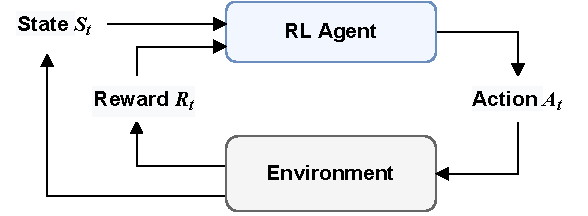
\includegraphics[width=0.7\textwidth]{RL-loop.pdf}
	\caption{Reinforcement Learning}
	\label{fig:RL-loop}
\end{figure}

Introduced in 1992, the REINFORCE algorithm \citep{REINFORCE-williams1992} is considered as a basic reinforcement learning algorithm. It is a policy-based, on-policy algorithm, capable of handling both discrete and continuous observation and action domains.

In practice the REINFORCE algorithm is considered as a ``weak" learner and superseded by several algorithms developed since. Most notably the Q-Learning and its deep-neural network version, the DQN \citep{DQN-mnih2013}, followed by Actor-Critic \citep{A2C-mnih2016} and one of the most robust modern-day algorithms, the PPO \citep{PPO-schulman2017}.

\subsection{Stable-Baselines3}
Stable-Baselines3 \cite{SB3-paper}, is Open Source and very popular among the RL community\footnote{As of 27-Jun-2023, it had 6k+ stars and 424 closed pull requests}. Stable-Baselines3 was initially based on the Open AI baselines \citep{OpenAI-baselines} and is completely rewritten using PyTorch. 


 for  , implementation s  the advanced algorithms -- DQN, A2C and PPO and compare its performance to a na\"ive custom implementation of the REINFORCE algorithm. We use Stable-Baselines3 (SB3), the highly popular and reliable implementations of DQN, A2C and PPO. As of 27-Jun-2023, the REINFORCE was not implemented by Stable-Baselines and we therefore custom implemented a basic version. 

\subsection{REINFORCE}
sB-3 dOES NOT IMPLEMENT THE REINFORCE	 --- https://stable-baselines3.readthedocs.io/en/master/guide/algos.html

Model Free --> Policy Gradient/Actor-Critic --> REINFORCE)
REINFORCE (Monte-Carlo policy gradient) 


IEEE NUAA Ideahouse dataset has been used in this paper for the RUL estimation of the milling cutter. \cite{NUAA-data-set}



Tool wear modeling is the first step to assist in predicting 


Literature search conducted on the Scopus\texttrademark{} and Web Of Science\texttrademark{} did not return any articles for the application of reinforcement learning for predictive maintenance of milling machines. Search strings we tried -- \texttt{``reinforcement learning AND tool wear AND maintenance", RL + milling + policy, RL + milling + maintenance, RL + tool wear + policy, RL + tool wear + maintenance"} 

Running the search \texttt{``reinforcement learning AND milling AND tool wear"} using the Scopus\texttrademark{} and Web Of Science\texttrademark{} services 

\cite{dai2021reinforcement} is the only article we found that tackles the 

Machine learning methods have been applied for example --
\cite{oshida2023development} proposes real-time tool wear detection during the milling process. They use a stacked LSTM encoder-decoder model for anomaly detection.


No results for "reinforcement learning" AND "milling machine" AND "tool wear" - on scopus or wos as of 23-jun-2023
"reinforcement learning" AND "milling machine" - 1 not relevant "	
\textit{Conference Paper}  •  Open access "Online Learning of Stability Lobe Diagrams in Milling" 	
Friedrich, J. Torzewski, J.  Verl, A.

"reinforcement learning" AND "tool wear" - 10 results


\section{Literature Review}

\section{Method}

\textit{The methodology explains in detail what the researcher did to undertake the research. Various aspects of the research have to be outlined: The overall structure and operation of the experiment or observational experience. The groups studied in the research including the size of each group and any features of the subjects which may be relevant to the topic being researched. The variables that were changed between groups and the variables measured as a result of the changes. The conditions under which the research was undertaken and any factors or variations in conditions which may have an impact on the results. The methods of data analysis used in order to analyse and collate the results. \textcolor{red}{***}Any limitations of the data collected.}
We normalize the tool wear and other state features, $x \in [0,\;1] \subset \mathbb{R} $. This allows for adding white noise of similar magnitudes across experiments of different data-sets
\subsection{RL environment description}
\subsection{Data description}
\subsection{Procedure}
 -- training \\
 -- selecting the model\\
 -- conducting the experiments\\
 
\subsection{Evaluation method}
\subsection{Tools}
2 different laptops

\begin{itemize}
	\item why classifction metrics
	\item why F1beta	
\end{itemize}

\subsection{Method - training and testing}
\subsection{Precision or Recall?}
- Precision => low FP => False replacement-action reduced. \textcolor{red}{***} Unnecessary tool replacement reduced. Tool life maximized, down time minimized, production disruption minimized \\
- Recall => low FN => False declaration of normal operation reduced. Reduce missed replacements. Tool replacements increased. \textcolor{red}{***} Product quality not compromised. 
\subsection{Hyper-parameters for Precision or Recall control}

\begin{itemize}
	\item R1 = +1 
	\item R2 = -1
	\item R3 = -100 => higher neg. Improve recall. Lower neg. Improve precision
	\item \textbf{LOOK AHEAD PARAM}: 
\end{itemize}

\begin{itemize}
	\item Training: SB3 - 10 k eps. 3 times. Average their outputs
	\item Testing: 
	\begin{itemize}
		\item Avg. over 5 rounds.
		\item Each round - avg over 40 test cases x 10 test rounds
		\item Total: 40 x 10 x 5 = 2000 cases
		\item Avgs over: 10 rounds (of 40 cases each) X 5 rounds of \textbf{re-trained} SB3 agents = 50 rounds 
	\end{itemize}
\end{itemize}

\subsection{Inference}
\begin{itemize}
	\item Training: SB3 is also unstable - show examples of results such as A2C/DQN 0.00 
	\item Training: SB3 is also unstable - SHOW SB3 tensorboard plots
	\item Training: SB3 is also unstable - EXCEL plots of results over the 10 rounds 	
\end{itemize}


\section{Network architecture and basic hyper-parameters}

\begin{table*}\centering
	\sffamily
	\rowspace{1.5}
	\begin{tabular}{L{2cm} R{2.5cm} R{2.5cm} R{2.5cm} R{3cm}}
		\arrayrulecolor{black!40}\toprule
		&\textbf{A2C}&\textbf{DQN}&\textbf{PPO}&\textbf{REINFORCE}\\ \midrule
		
		Network\par architecture&input dim x\par [64|Tanh x 64|Tanh]\par x output dim&input dim x\par [64|Tanh x 64|Tanh]\par x output dim&input dim x\par [64|Tanh x 64|Tanh]\par x output dim&input dim x\par [64|ReLU]\par x output dim\\
		Layers&2&2&2&1\\
		Units&64  x 64&64  x 64&64  x 64&64\\
		Activation&Tanh, Tanh&Tanh, Tanh&Tanh, Tanh&ReLU\\
		Optimizer&RMSprop&Adam&Adam&Adam\\ \midrule
		Learning rate&0.0007&0.0001&0.0003&0.01\\
		Gamma&0.99&0.99&0.99&0.99\\			
		\bottomrule
	\end{tabular}
	\caption{Comparing the network architecture and basic hyper-parameters across algorithms}
	\label{tbl:hyperparameters}
\end{table*}




soure of ppo implementation details \url{https://iclr-blog-track.github.io/2022/03/25/ppo-implementation-details/}

source of SB3 network mp : \url{https://github.com/openai/baselines/blob/ea25b9e8b234e6ee1bca43083f8f3cf974143998/baselines/common/models.py#L75-L103}

\subsection{PPO hyperparms}

implementation guide source >> https://iclr-blog-track.github.io/2022/03/25/ppo-implementation-details/

By default, PPO uses a simple MLP network consisting of two layers of 64 neurons and Hyperbolic Tangent as the activation function. Then PPO builds a policy head and value head that share the outputs of the MLP network. Below is a pseudocode:
%\textt{
%network = Sequential(
%layer_init(Linear(np.array(envs.single_observation_space.shape).prod(), 64)),
%Tanh(),
%layer_init(Linear(64, 64)),
%Tanh(),
%)
%value_head = layer_init(Linear(64, 1), std=1.0)
%policy_head = layer_init(Linear(64, envs.single_action_space.n), std=0.01)
%hidden = network(observation)
%value = value_head(hidden)
%action = Categorical(policy_head(hidden)).sample()}

\subsection{dqn hyperparms}


default hyperparms : \url{https://stable-baselines3.readthedocs.io/en/master/_modules/stable_baselines3/common/policies.html}

overridden in indiv policies for example 
SB3 DQN hypoerparms for example were taken from ;
Paper: https://arxiv.org/abs/1312.5602, https://www.nature.com/articles/nature14236
Default hyperparameters are taken from the Nature paper,
except for the optimizer and learning rate that were taken from Stable Baselines defaults




\section{Empirical results}

\begin{figure}[ht]
	\begin{subfigure}{\textwidth}
	\centering
	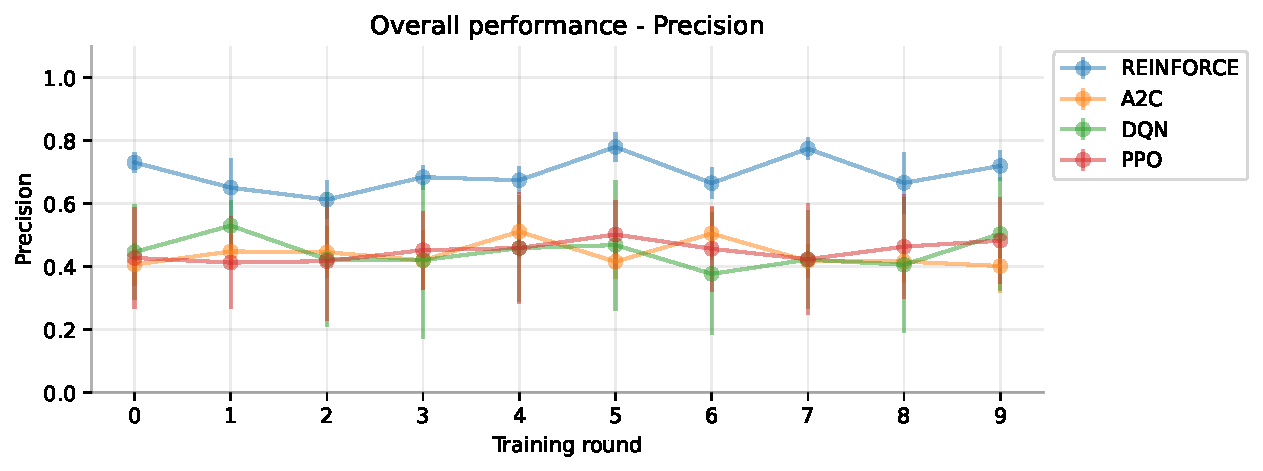
\includegraphics[width=\linewidth]{Overall_Pr.pdf}  
	\caption{Precision}
	\label{fig:tr-ovr-pr}
	\end{subfigure} \par\smallskip

	\begin{subfigure}{\textwidth}
	\centering
	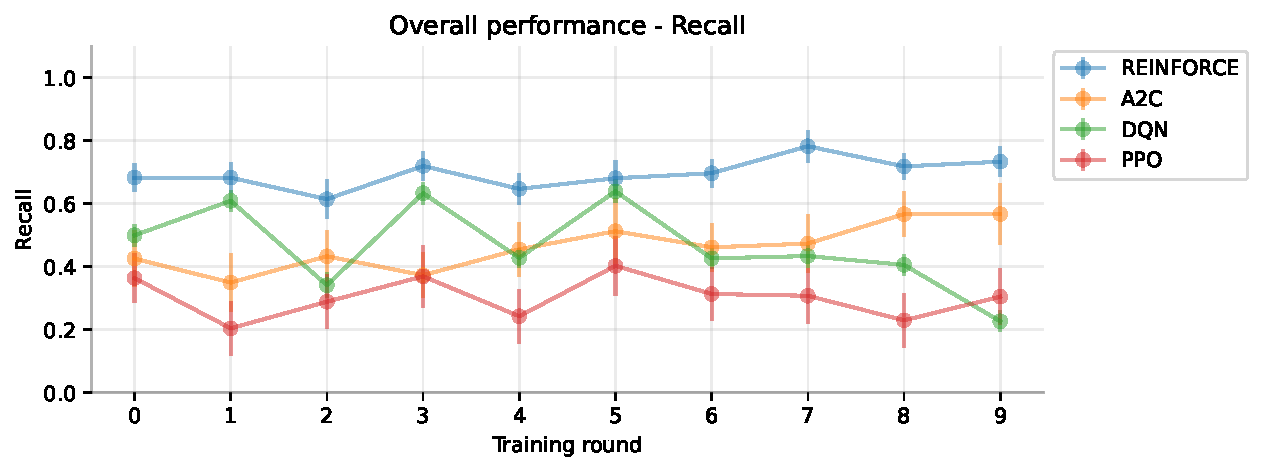
\includegraphics[width=\linewidth]{Overall_Rc.pdf}  
	\caption{Recall}
	\label{fig:tr-ovr-rc}
	\end{subfigure} \par\smallskip
	
	\begin{subfigure}{\textwidth}
		\centering
		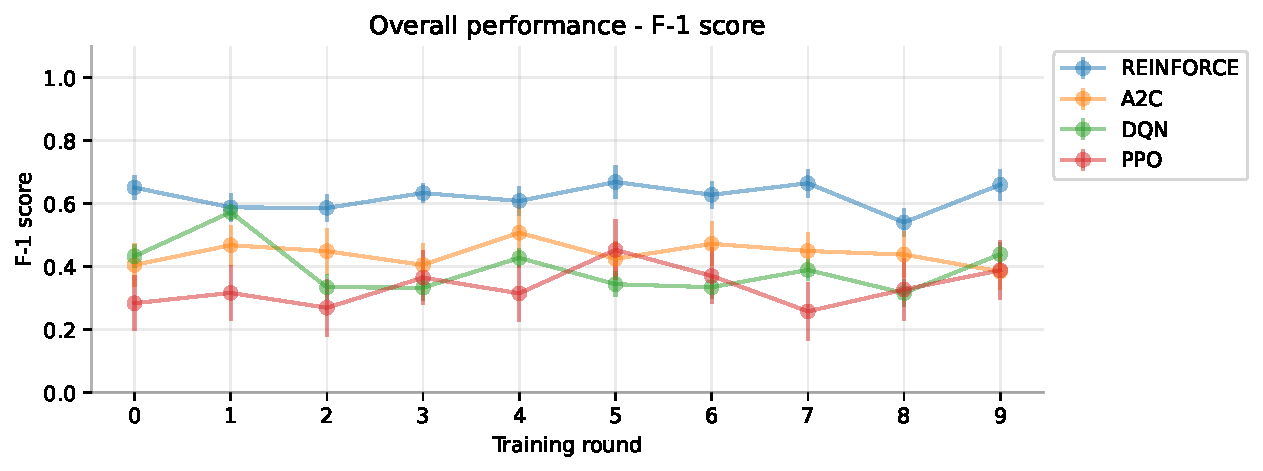
\includegraphics[width=\linewidth]{Overall_F1.pdf}  
		\caption{F1-score}
		\label{fig:tr-ovr-f1}
	\end{subfigure} \par\smallskip

	\begin{subfigure}{\textwidth}
		\centering
		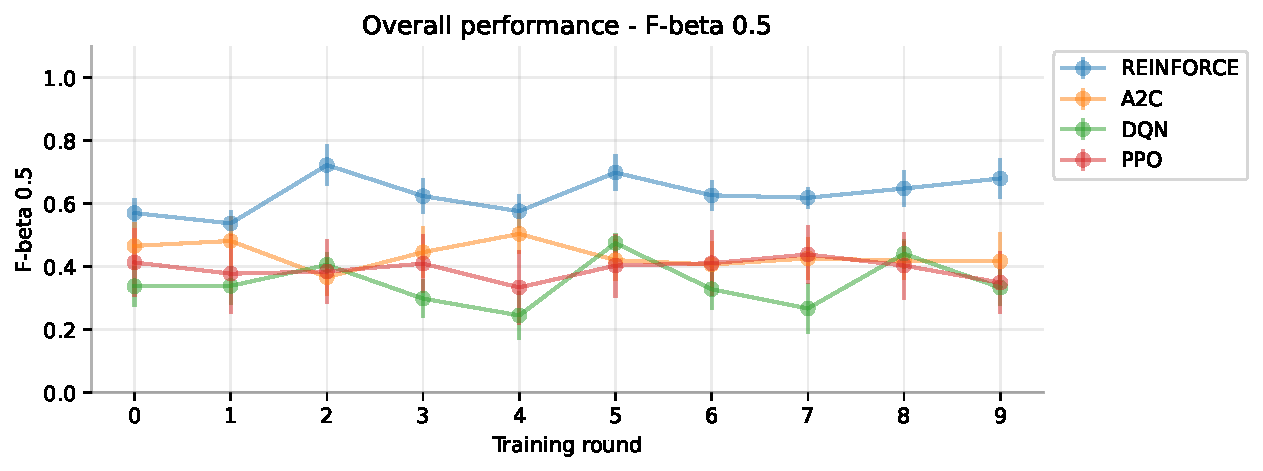
\includegraphics[width=\linewidth]{Overall_F05.pdf}  
		\caption{F1-beta (0.5)}
		\label{fig:tr-ovr-f05}
	\end{subfigure}
	\caption{Overall performance -- Metrics across 10 rounds of model training}
	\label{fig:tr-overall}
\end{figure}

\begin{figure}[ht]
	\begin{subfigure}{\textwidth}
		\centering
		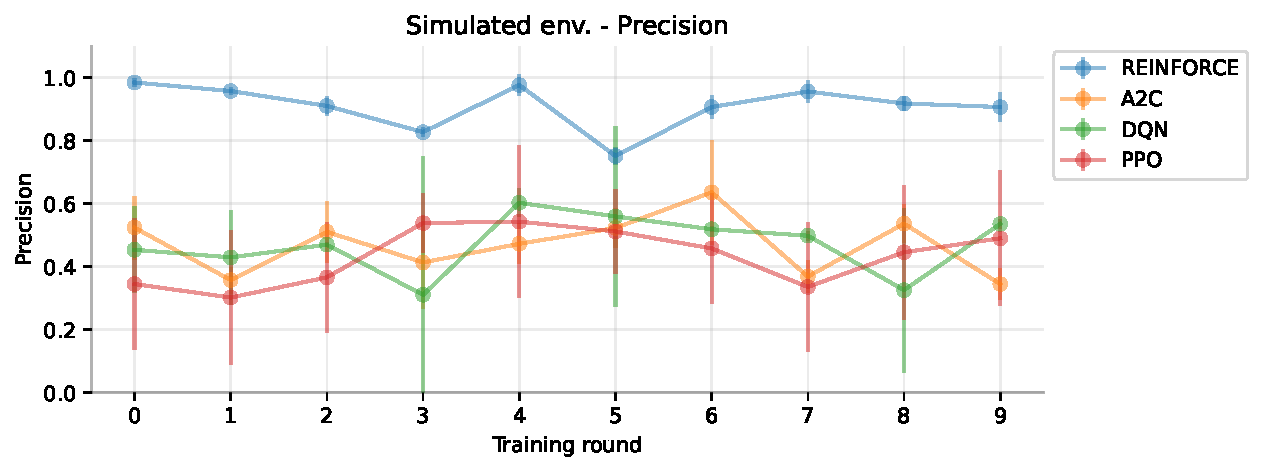
\includegraphics[width=\linewidth]{Simulated_Pr.pdf}  
		\caption{Precision}
		\label{fig:tr-sim-pr}
	\end{subfigure} \par\smallskip
	
	\begin{subfigure}{\textwidth}
		\centering
		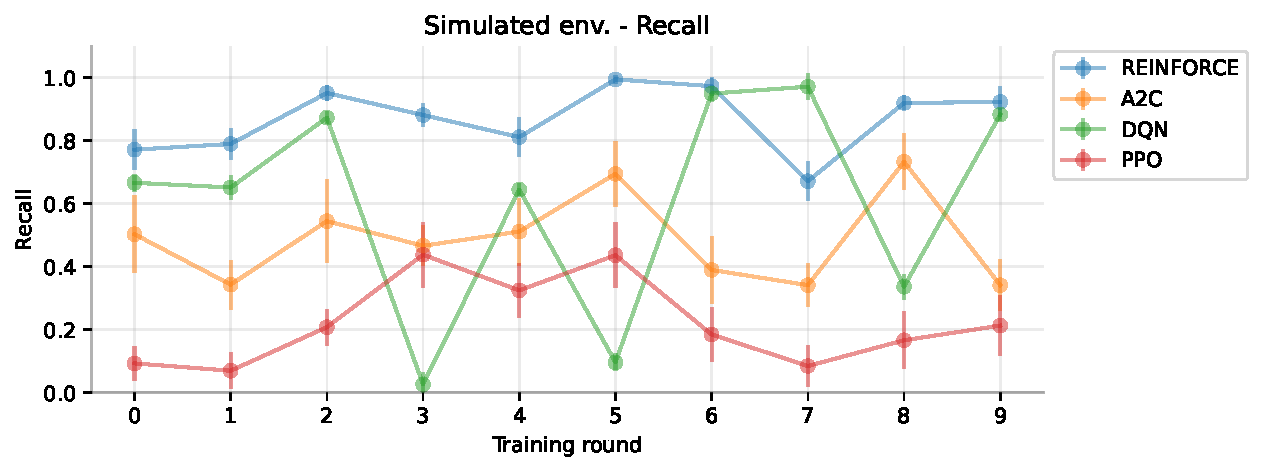
\includegraphics[width=\linewidth]{Simulated_Rc.pdf}  
		\caption{Recall}
		\label{fig:tr-sim-rc}
	\end{subfigure} \par\smallskip
	
	\begin{subfigure}{\textwidth}
		\centering
		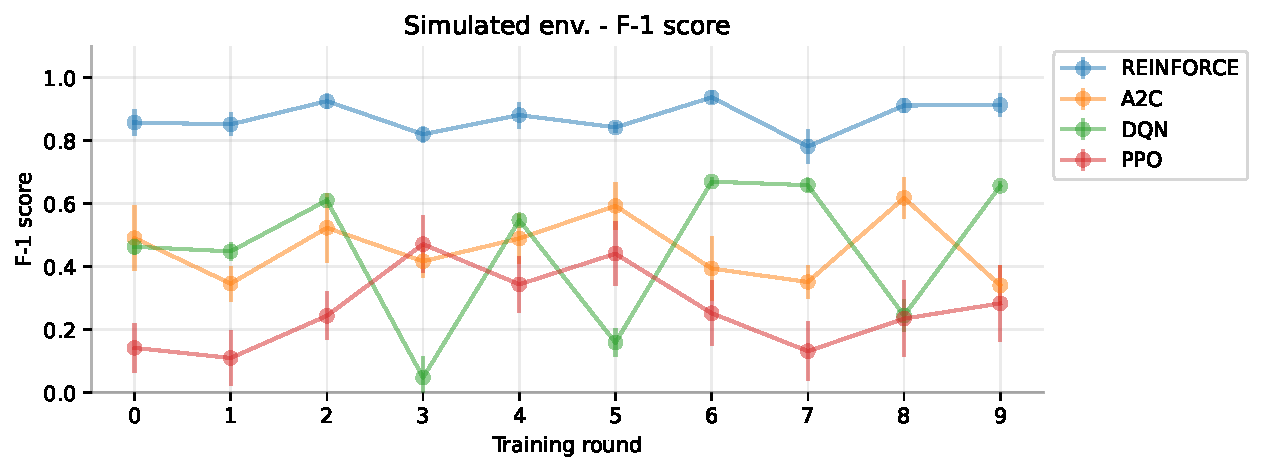
\includegraphics[width=\linewidth]{Simulated_F1.pdf}  
		\caption{F1-score}
		\label{fig:tr-sim-f1}
	\end{subfigure} \par\smallskip
	
	\begin{subfigure}{\textwidth}
		\centering
		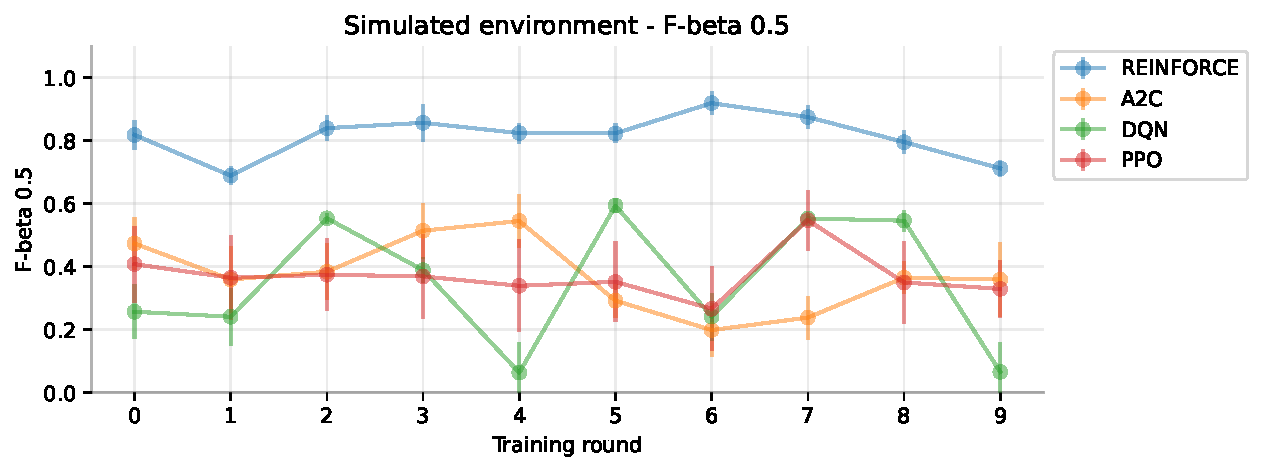
\includegraphics[width=\linewidth]{Simulated_F05.pdf}  
		\caption{F1-beta (0.5)}
		\label{fig:tr-sim-f05}
	\end{subfigure}
	\caption{Simulated environment -- Metrics across 10 rounds of model training}
	\label{fig:tr-sim-env}
\end{figure}

\begin{figure}[ht]
	\begin{subfigure}{\textwidth}
		\centering
		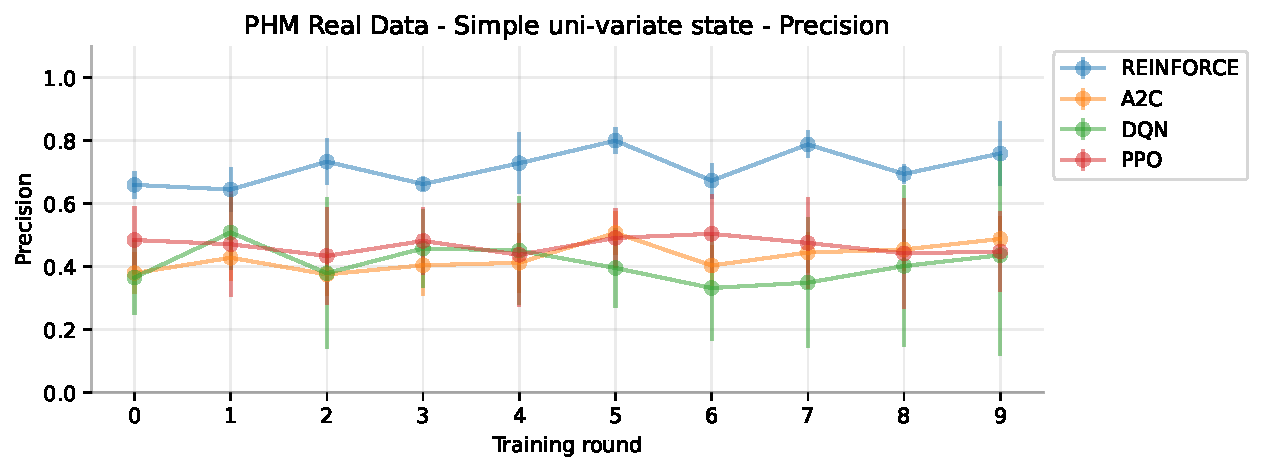
\includegraphics[width=\linewidth]{Singevariable_Pr.pdf}  
		\caption{Precision}
		\label{fig:tr-ss-pr}
	\end{subfigure} \par\smallskip
	
	\begin{subfigure}{\textwidth}
		\centering
		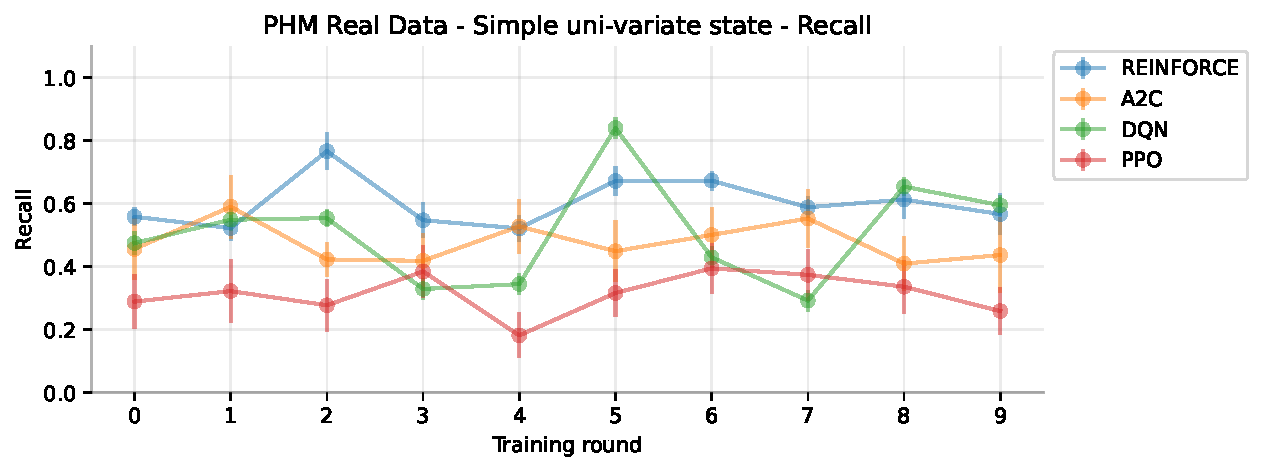
\includegraphics[width=\linewidth]{Singevariable_Rc.pdf}  
		\caption{Recall}
		\label{fig:tr-ss-rc}
	\end{subfigure} \par\smallskip
	
	\begin{subfigure}{\textwidth}
		\centering
		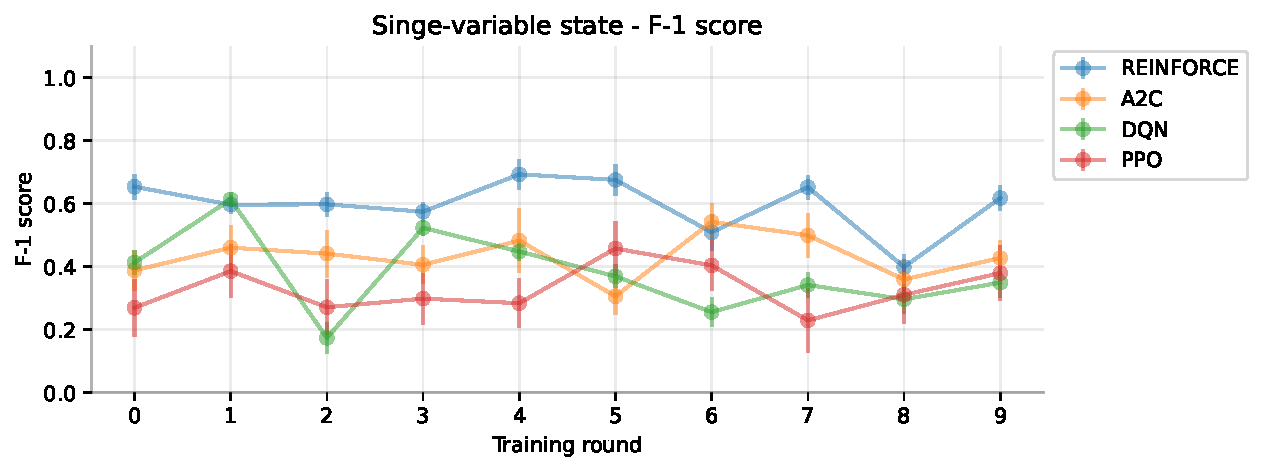
\includegraphics[width=\linewidth]{Singevariable_F1.pdf}  
		\caption{F1-score}
		\label{fig:tr-ss-f1}
	\end{subfigure} \par\smallskip
	
	\begin{subfigure}{\textwidth}
		\centering
		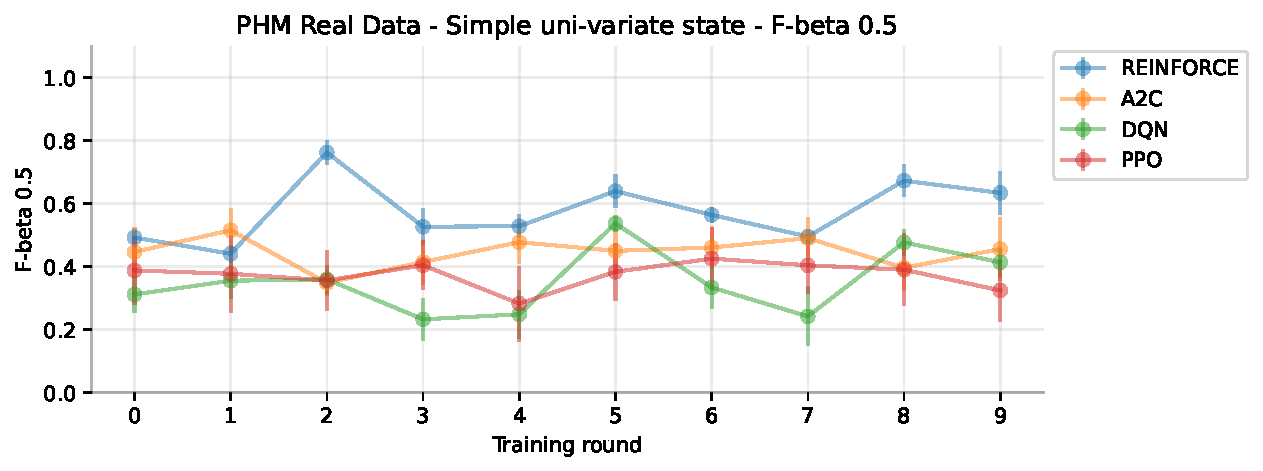
\includegraphics[width=\linewidth]{Singevariable_F05.pdf}  
		\caption{F1-beta (0.5)}
		\label{fig:tr-ss-f05}
	\end{subfigure}
	\caption{Singe-variable state environment -- Metrics across 10 rounds of model training}
	\label{fig:tr-ss-env}
\end{figure}

\begin{figure}[ht]
	\begin{subfigure}{\textwidth}
		\centering
		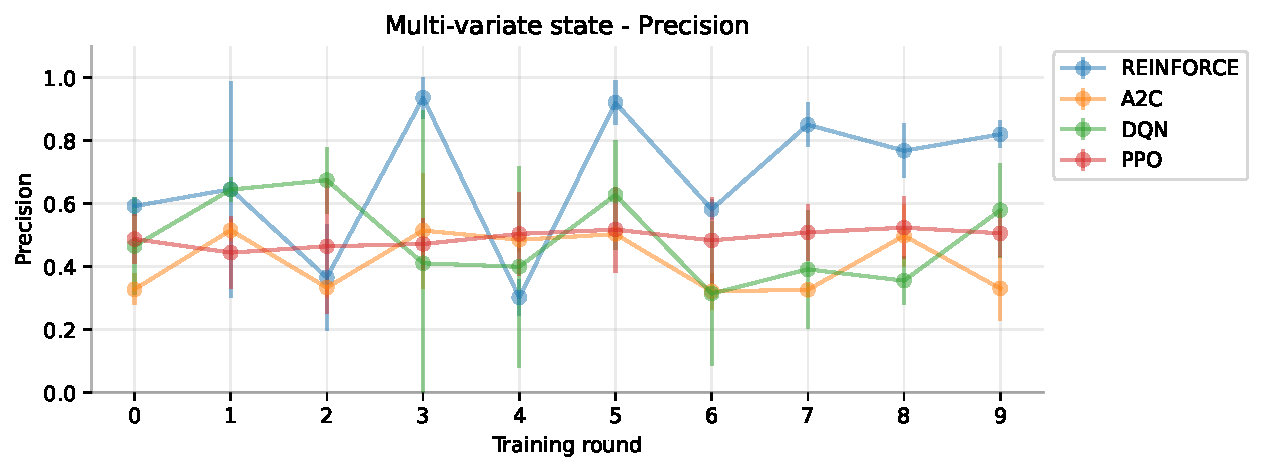
\includegraphics[width=\linewidth]{Multivariate_Pr.pdf}  
		\caption{Precision}
		\label{fig:tr-ms-pr}
	\end{subfigure} \par\smallskip
	
	\begin{subfigure}{\textwidth}
		\centering
		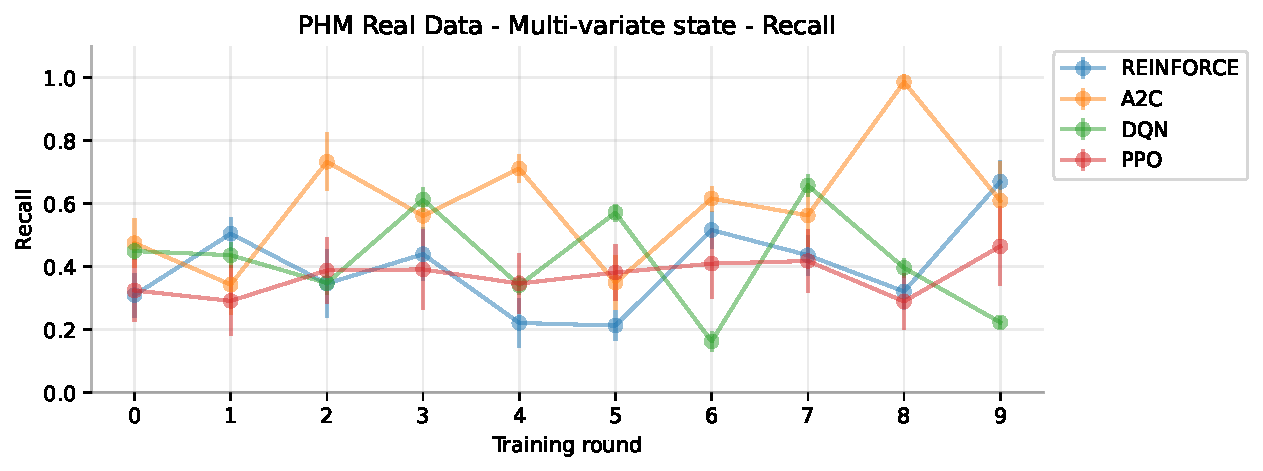
\includegraphics[width=\linewidth]{Multivariate_Rc.pdf}  
		\caption{Recall}
		\label{fig:tr-ms-rc}
	\end{subfigure} \par\smallskip
	
	\begin{subfigure}{\textwidth}
		\centering
		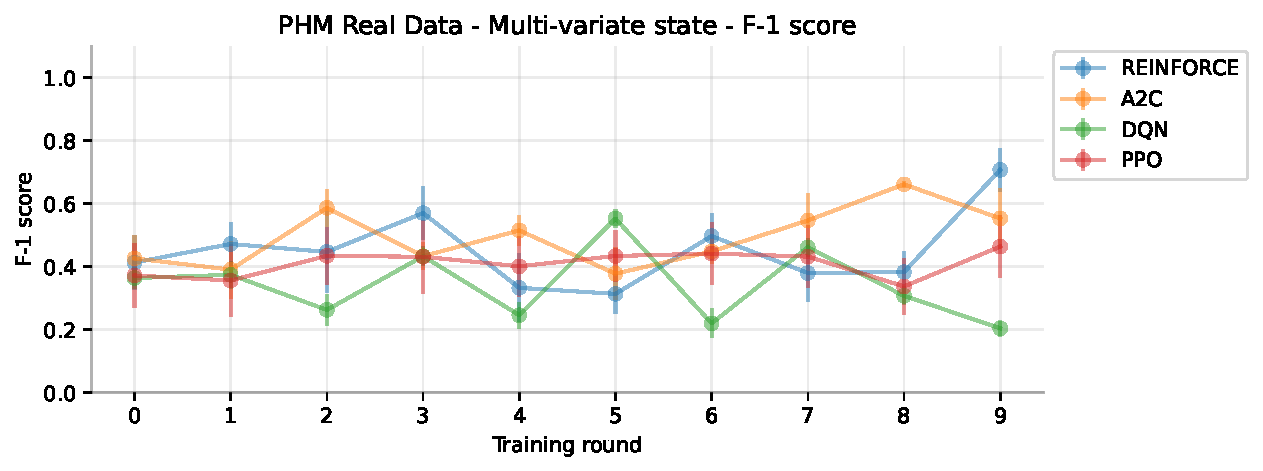
\includegraphics[width=\linewidth]{Multivariate_F1.pdf}  
		\caption{F1-score}
		\label{fig:tr-ms-f1}
	\end{subfigure} \par\smallskip
	
	\begin{subfigure}{\textwidth}
		\centering
		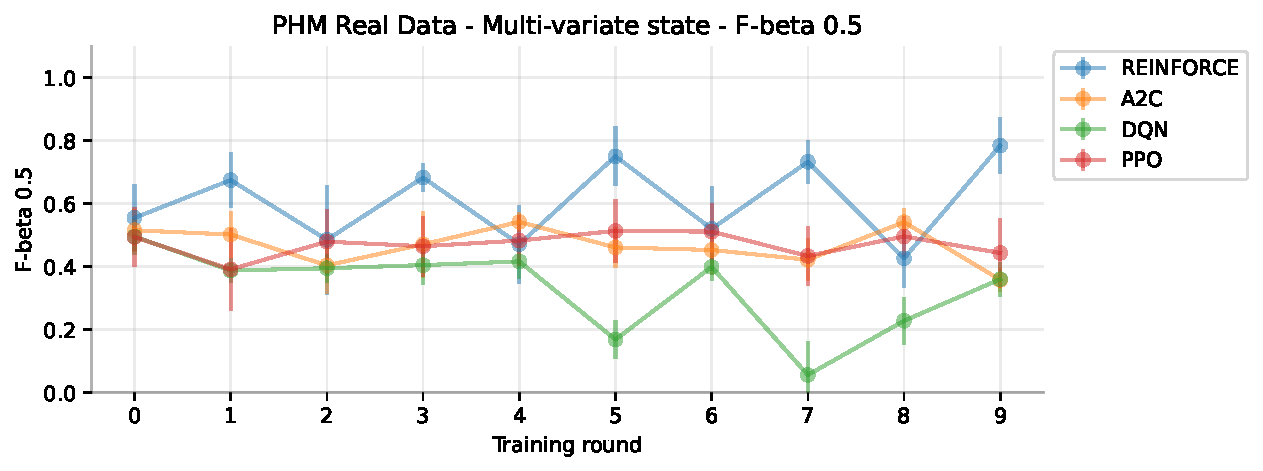
\includegraphics[width=\linewidth]{Multivariate_F05.pdf}  
		\caption{F1-beta (0.5)}
		\label{fig:tr-ms-f05}
	\end{subfigure}
	\caption{Multi-variate state environment -- Metrics across 10 rounds of model training}
	\label{fig:tr-ms-env}
\end{figure}


\subsection{Detailed metrics}
\newgeometry{margin=2cm} % Change margins for landscape table
\begin{landscape}\centering
	\begin{table*}
		\sffamily
		\rowspace{1.3}
		\begin{tabular}{@{}l rrrr c rrrr c rrrr c rrrr@{}} \arrayrulecolor{black!40}\toprule
			& \multicolumn{4}{c}{\textbf{REINFORCE}} & & \multicolumn{4}{c}{A2C} &
			& \multicolumn{4}{c}{DQN} & & \multicolumn{4}{c}{PPO} \\
			\cmidrule{2-5} \cmidrule{7-10} \cmidrule{12-15} \cmidrule{17-20}
			Environment &Prec. &Recall &F1 &F0.5 & &Prec. &Recall &F1 &F0.5 & &Prec. &Recall &F1 &F0.5 & &Prec. &Recall &F1 &F0.5\\ \midrule
			
			Simulated  - No noise &0.999 &0.645 &0.782 & 0.898 & & 0.335 &0.359 &0.344 &0.338 & &0.348 &0.597 &0.410 &0.352 & &0.392 &0.211 &0.252&0.303\\
			Simulated  - Low noise &0.943 &0.954 &0.948 & 0.945 & & 0.409 &0.318 &0.349 &0.379 & &0.273 &0.064 &0.076 &0.108 & &0.359 &0.173 &0.205&0.255\\
			Simulated  - High noise &0.889 &0.974 &0.929 & 0.904 & & 0.471 &0.439 &0.443 &0.455 & &0.423 &0.408 &0.295 &0.284 & &0.402 &0.205 &0.248&0.307\\ \midrule
			
			PHM C01 SS - No noise &0.886 &0.978 &0.928 & 0.902 & & 0.294 &0.337 &0.305 &0.296 & &0.350 &0.405 &0.291 &0.269 & &0.517 &0.494 &0.471&0.476\\
			PHM C01 SS - Low noise &0.916 &0.893 &0.903 & 0.911 & & 0.526 &0.645 &0.568 &0.540 & &0.321 &0.591 &0.404 &0.343 & &0.490 &0.415 &0.443&0.468\\
			PHM C01 SS - High noise &0.757 &0.926 &0.831 & 0.784 & & 0.499 &0.632 &0.542 &0.513 & &0.399 &0.402 &0.308 &0.292 & &0.403 &0.223 &0.270&0.325\\ \hdashline
			
			PHM C04 SS - No noise &0.865 &0.959 &0.908 & 0.881 & & 0.515 &0.676 &0.575 &0.535 & &0.365 &0.497 &0.383 &0.348 & &0.431 &0.239 &0.265&0.311\\
			PHM C04 SS - Low noise &0.722 &0.980 &0.831 & 0.762 & & 0.399 &0.393 &0.391 &0.393 & &0.409 &0.589 &0.410 &0.361 & &0.438 &0.299 &0.334&0.377\\
			PHM C04 SS - High noise &0.770 &0.809 &0.787 & 0.776 & & 0.375 &0.456 &0.397 &0.381 & &0.408 &0.411 &0.296 &0.282 & &0.491 &0.324 &0.362&0.409\\ \hdashline
			
			PHM C06 SS - No noise &0.996 &0.609 &0.751 & 0.879 & & 0.463 &0.454 &0.455 &0.459 & &0.538 &0.780 &0.585 &0.523 & &0.402 &0.410 &0.374&0.370\\
			PHM C06 SS - Low noise &0.968 &0.854 &0.905 & 0.941 & & 0.508 &0.615 &0.548 &0.522 & &0.395 &0.593 &0.411 &0.362 & &0.454 &0.342 &0.367&0.404\\
			PHM C06 SS - High noise &0.699 &0.912 &0.790 & 0.732 & & 0.480 &0.512 &0.466 &0.467 & &0.581 &0.499 &0.417 &0.433 & &0.424 &0.199 &0.252&0.314\\ \midrule
			
			PHM C01 MS - No noise &0.824 &0.895 &0.856 & 0.836 & & 0.444 &0.284 &0.315 &0.358 & &0.313 &0.215 &0.165 &0.175 & &0.513 &0.347 &0.395&0.448\\
			PHM C04 MS - No noise &0.752 &0.678 &0.709 & 0.733 & & 0.506 &0.326 &0.368 &0.425 & &0.588 &0.642 &0.492 &0.486 & &0.472 &0.455 &0.444&0.452\\
			PHM C06 MS - No noise &1.000 &0.643 &0.779 & 0.896 & & 0.499 &0.731 &0.575 &0.523 & &0.520 &0.239 &0.209 &0.256 & &0.509 &0.260 &0.330&0.409\\
					
			\bottomrule
		\end{tabular}
		\caption{Model performance comparison all variants of the environments.}
		\label{tbl:DetailedMetrics}
	\end{table*}
\end{landscape}
\restoregeometry % Restore margins after landscape table

\subsection{Overall summary performance}
\begin{table*}[hbt!]\centering
	\sffamily
	\rowspace{1.3}
	\begin{tabular}{@{}l rr c rr c rr c rr@{}}
		\arrayrulecolor{black!40}\toprule
		& \multicolumn{2}{c}{Precision} & \phantom{i} & \multicolumn{2}{c}{Recall} & \phantom{i} & \multicolumn{2}{c}{F1-score} & \phantom{i} & \multicolumn{2}{c}{F1-beta score} \\
		\cmidrule{2-3} \cmidrule{5-6} \cmidrule{8-9} \cmidrule{11-12} 
		
		&Mean &SD & &Mean &SD & &Mean &SD& &Mean & SD\\ \midrule
		A2C & 0.448 & 0.074 & &0.478 & 0.084 & & 0.443 & 0.071 & &0.439 &0.069 \\
		DQN & 0.415 & 0.196 & &0.462 & 0.033 & & 0.343 & 0.038 & &0.325 &0.063 \\
		PPO & 0.447 & 0.147 & &0.306 & 0.090 & & 0.334 & 0.093 & &0.375 &0.107 \\
		REINFORCE & 0.866 & 0.042 & &0.847 & 0.054 & & 0.842 & 0.043 & &0.852 &0.042 \\	
		\bottomrule
	\end{tabular}
	\caption{Model performance summary - averaged over all environment.}
	\label{tbl:OverallSummary}
\end{table*}

\subsection{Simulated environment}
\begin{table*}[hbt!]\centering\sffamily
	\rowspace{1.3}
	\begin{tabular}{@{}l rr c rr c rr c rr@{}}
		\arrayrulecolor{black!40}\toprule
		& \multicolumn{2}{c}{Precision} & \phantom{i} & \multicolumn{2}{c}{Recall} & \phantom{i} & \multicolumn{2}{c}{F1-score} & \phantom{i} & \multicolumn{2}{c}{F1-beta score} \\
		\cmidrule{2-3} \cmidrule{5-6} \cmidrule{8-9} \cmidrule{11-12} 
		
		&Mean &SD & &Mean &SD & &Mean &SD& &Mean & SD\\ \midrule
		A2C & 0.405 & 0.079 & &0.372 & 0.086 & & 0.379 & 0.076 & &0.391 &0.076 \\
		DQN & 0.348 & 0.217 & &0.356 & 0.033 & & 0.260 & 0.041 & &0.248 &0.068 \\
		PPO & 0.385 & 0.175 & &0.196 & 0.064 & & 0.235 & 0.080 & &0.289 &0.110 \\
		REINFORCE & 0.944 & 0.029 & &0.858 & 0.041 & & 0.886 & 0.032 & &0.916 &0.030 \\
		\bottomrule
	\end{tabular}
	\caption{Model performance summary - averaged over simulated environments.}
	\label{tbl:SimulatedEnv}
\end{table*}

\newpage
\subsection{Real data -- simple single-variable environment}
\begin{table*}[h]\centering
	\sffamily
	\rowspace{1.3}
	\begin{tabular}{@{}l rr c rr c rr c rr@{}}
		\arrayrulecolor{black!40}\toprule
		& \multicolumn{2}{c}{Precision} & \phantom{i} & \multicolumn{2}{c}{Recall} & \phantom{i} & \multicolumn{2}{c}{F1-score} & \phantom{i} & \multicolumn{2}{c}{F1-beta score} \\
		\cmidrule{2-3} \cmidrule{5-6} \cmidrule{8-9} \cmidrule{11-12} 
		
		&Mean &SD & &Mean &SD & &Mean &SD& &Mean & SD\\ \midrule
		A2C & 0.451 & 0.064 & &0.524 & 0.085 & & 0.472 & 0.067 & &0.456 &0.063 \\
		DQN & 0.418 & 0.172 & &0.530 & 0.032 & & 0.389 & 0.034 & &0.357 &0.055 \\
		PPO & 0.450 & 0.146 & &0.327 & 0.095 & & 0.349 & 0.095 & &0.384 &0.106 \\
		REINFORCE & 0.842 & 0.043 & &0.880 & 0.053 & & 0.848 & 0.043 & &0.841 &0.042 \\
		\bottomrule
	\end{tabular}
	\caption{Model performance summary - averaged over PHM-2010 environments with simple single-variable environment.}
	\label{tbl:PHMSS}
\end{table*}

\subsection{Real data -- complex multi-variate environment}
\begin{table*}[hbt!]\centering
	\sffamily
	\rowspace{1.3}
	\begin{tabular}{@{}l rr c rr c rr c rr@{}}
		\arrayrulecolor{black!40}\toprule
		& \multicolumn{2}{c}{Precision} & \phantom{i} & \multicolumn{2}{c}{Recall} & \phantom{i} & \multicolumn{2}{c}{F1-score} & \phantom{i} & \multicolumn{2}{c}{F1-beta score} \\
		\cmidrule{2-3} \cmidrule{5-6} \cmidrule{8-9} \cmidrule{11-12} 
		
		&Mean &SD & &Mean &SD & &Mean &SD& &Mean & SD\\ \midrule
		A2C & 0.483 & 0.101 & &0.447 & 0.081 & & 0.419 & 0.075 & &0.435 &0.079 \\
		DQN & 0.474 & 0.248 & &0.365 & 0.038 & & 0.289 & 0.049 & &0.306 &0.082 \\
		PPO & 0.498 & 0.121 & &0.354 & 0.103 & & 0.390 & 0.101 & &0.436 &0.104 \\
		REINFORCE & 0.859 & 0.053 & &0.739 & 0.069 & & 0.781 & 0.055 & &0.822 &0.052 \\
		\bottomrule
	\end{tabular}
	\caption{Model performance summary - averaged over PHM-2010 environments with complex multi-variate environment.}
	\label{tbl:PHMMS}
\end{table*}

\subsection{Training times}

\begin{table*}[hbt!]\centering
	\sffamily
	\rowspace{1.3}
	\begin{tabular}{@{}l r r r r@{}}
		\arrayrulecolor{black!40}\toprule
		\textbf{Environment} &\textbf{REINFORCE} &\textbf{A2C}&\textbf{DQN}&\textbf{PPO}\\ \midrule
		Simulated  - No noise &214.23 &41.19&4.03&41.13\\
		Simulated  - Low noise &199.89 &41.52&3.55&40.66\\
		Simulated  - High noise &134.16 &17.88&1.53&20.90\\ \midrule
		
		PHM C01 SS - No noise &330.54 &18.85&2.08&32.65\\
		PHM C01 SS - Low noise &426.79 &30.66&3.69&38.59\\
		PHM C01 SS - High noise &333.13 &17.58&1.80&19.16\\ \midrule
		
		PHM C04 SS - No noise &299.31 &19.56&1.86&19.64\\
		PHM C04 SS - Low noise &264.90 &18.27&2.00&19.69\\
		PHM C04 SS - High noise &256.44 &17.65&1.58&19.11\\ \hdashline
		
		PHM C06 SS - No noise &339.65 &17.64&2.26&19.50\\
		PHM C06 SS - Low noise &266.98 &19.33&1.84&19.19\\
		PHM C06 SS - High noise &308.20 &34.21&4.18&30.94\\ \hdashline
		
		PHM C01 MS - No noise &655.21 &38.55&4.96&42.21\\
		PHM C04 MS - No noise &615.58 &33.85&7.36&43.49\\
		PHM C06 MS - No noise &625.37 &39.30&5.85&41.68\\  \midrule
		
		Overall average (s) &351.36 &27.07&3.24&29.90\\
		\bottomrule
\end{tabular}
\caption{Training time for each model, across different environments. Averaged over 3 runs. Time is in seconds (s).}
\label{tbl:TrainingTimes}
\end{table*}

%\subsection{Algorithm timelines}
%\begin{itemize}
%	\item 1947: Monte Carlo Sampling
%	\item 1959: Temporal Difference Learning
%	\item 1989: Q-Learning
%	\item 1992: REINFORCE
%	\item 2013: DQN
%	\item 2016: A3C
%	\item 2017: PPO 
%\end{itemize}

\section{The REINFORCE algorithm}
Three key features of any RL algorithm:
\begin{enumerate}
	\item Policy: $\pi_\theta$ = Probablities of all actions, given a state. Parameterized by $\theta$
	\item Objective function:
	\begin{equation}
		\max_{\theta} J(\pi_{\theta}) = \mathop{\mathbb{E}}_{\tau \sim \pi_\theta} [R(\tau)]
	\end{equation}
	\item Method: Way to udate the parameters = Policy Gradient

\end{enumerate}

\subsection{Policy gradient numerical computation}

\begin{enumerate}
	\item Plain vanilla: 
	\begin{equation}
		\nabla \theta J(\pi_\theta) = \mathbb{E}_{\tau \sim \pi_\theta} \; [ \; \sum_{t=0}^T R_t(\tau) \; \nabla_\theta \ln \pi_\theta(a_t \vert s_t) \;]
	\end{equation}
	\item With Monte Carlo sampling and approximation: $\nabla_\theta J(\pi_\theta) \approx [ \; \sum_{t=0}^T R_t(\tau) \; \nabla_\theta \ln \pi_\theta(a_t \vert s_t) \;]$
	\item With baseline: $\nabla_\theta J(\theta) \approx [ \; \sum_{t=0}^T (R_t(\tau) - b(s_t)) \; \nabla_\theta \ln \pi_\theta(a_t \vert s_t) \;]$
	\item Where, baseline does not change per time-step, it is for the entire trajectory
	\item One baseline option: $V^\pi$ - leads to Actor-Critic algorithm
	\item Simpler option: Average returns over trajectory: $b = \frac{1}{T}\sum_{t=0}^T R_t(\tau) $
\end{enumerate}

Algorithm
%1. Initialize $\alpha$, $\gamma$ and $\theta$ i.e. weigths of the NN
%2. for episodes = 0 to MAX_EPISODES:
%- sample trajectory $\tau$
%- set $\nabla_\theta J(\pi_{\theta})$ = 0
%- for t=0 to T:
%- $R_t(\tau) = \sum_{t'=t}^{T} \gamma^{t'-t} r'_t$
%- $\nabla_\theta J(\pi_\theta)  = \mathbb{E}_{\tau \sim \pi_\theta} \; [ \; \sum_{t=0}^T R_t(\tau) \; \nabla_\theta \ln \pi_\theta(a_t \vert s_t) \;]$
%- end for sampled trajectory
%- $\theta = \theta + \alpha \nabla_\theta J(\pi_\theta) $
%3. end for all episodes 
%
%Implementation notes:
%1. Code is inspired by Laura Graesser's (LG, 2020 book) implementation, however with large modifications
%2. We use the concept of Agent (instead of 'pi' or '$policy_pi$') and a separate network class (i.e. how the function approximator is implemented, it could well be a linear regression)
%3. **Important concept**: "Loss" in the implementation below, is the "objective" $J$. In our algorithm, we want to **maximize** it. PyTorch's optimizer, by default, MINIMIZES it (as it is called "loss"), we therefore add "-" negate it, so as to maximize it. 
%4. Also in the final plot, notice "loss" is RISING and follows the rewards, which is expected as "loss" is really being maximized.  
%5. self.pd.probs = prob. distribution of all actions
%6. Sum of all possible action probabilities = 1.0
%7. Note that episodes > 300 start showing repeated patterns. Rewards drop and rise in cylces. 300 is ideal and hence suggested in LG (2020)



\section{Discussion}

\subsection{Precision or Recall?}
- Precision => low FP => False replacement-action reduced. \textcolor{red}{***} Unnecessary tool replacement reduced. Tool life maximized, down time minimized, production disruption minimized \\
- Recall => low FN => False declaration of normal operation reduced. Reduce missed replacements. Tool replacements increased. \textcolor{red}{***} Product quality not compromised. 


limitiongs of the slecting model for evaluation

\cite{SB3-paper} -- quote from paper - intro section -- "A major challenge is that small implementation details can have a substantial effect on performance often greater than the difference between algorithms (Engstrom et al., 2020). It is particularly important that  implementations used as experimental baselines are reliable; otherwise, novel algorithms compared to weak baselines lead to inated estimates of performance improvements"

DPO paper - Rafael Rafailov May-2023 --- Direct Preference Optimization: Your Language Model is Secretly a Reward Model 

5.2 Instability of Actor-Critic Algorithms
We can also use our framework to diagnose instabilities with standard actor-critic algorithms used
for the RLHF, such as PPO. We follow the RLHF pipeline and focus on the RL fine-tuning step
outlined in Section 3. We can draw connections to the control as inference framework [18] for the
constrained RL problem outlined in 3. We assume a parameterized model and minimize
This is the same objective optimized in prior works [45, 35, 1, 23] using the DPO-equivalent reward
for the reward class of In this setting, we can interpret the normalization term in 
as the soft value function of the reference policy . While this term does not affect the optimal
solution, without it, the policy gradient of the objective could have high variance, making learning
unstable. We can accommodate for the normalization term using a learned value function, but that
can also be difficult to optimize. Alternatively, prior works have normalized rewards using a human
completion baseline, essentially a single sample Monte-Carlo estimate of the normalizing term. In
contrast the DPO reparameterization yields a reward function that does not require any baselines.

\section{Conclusion}


%% References
\bibliography{ES_bibliography}
\end{document}
